%!TEX output_directory=output
\documentclass[twocolumn, aps, 10pt]{revtex4-2}

\usepackage[revtex]{kaufman}

\begin{document}

%\preprint{IDK...}
% TODO what does this do?

\title{Reinforcement Learning for Hamiltonian Engineering}
%\thanks{Ramanathan Lab}
\author{Will Kaufman}
\affiliation{%
Dartmouth College, Ramanathan Lab}
\date{September 14, 2020}

% TODO include abstract?

\maketitle


\section{Hamiltonian Engineering and Average Hamiltonian Theory}

The time evolution of a quantum system depends on the system's Hamiltonian. For a system with initial density operator $\rho(0)$ and Hamiltonian $H(t)$, the state at time $t$ is given by
\[
\rho(t) = U(t)\rho(0)U^\dagger(t)
\]
where the propagator $U(t)$ maps from initial states ($t=0$) to states at time $t$. $U(t)$ is determined by the propagator Schrödinger equation
\begin{equation}\label{eq:time_evolution_diff_eq}
    \ddt{U(t)} = \frac{-i}{\hbar} H(t) U(t), U(0) = \identity
\end{equation}
The total Hamiltonian can be broken into a time-independent system Hamiltonian and a time-dependent control Hamiltonian.
\begin{equation}
    H(t) = H_\text{sys} + H_c(t)
\end{equation}
\emph{Hamiltonian engineering} seeks to design the time-dependent Hamiltonian $H_c(t)$ to control the system's evolution so that it appears to evolve under a target ``effective'' Hamiltonian ($H_\text{target}$) when measured stroboscopically. That is,
\begin{equation}\label{eq:strob_measure}
    \rho(NT) = U_\text{target}(NT) \rho(0) U_\text{target}^\dagger(NT)
\end{equation}
where $U_\text{target}$ is the propagator determined by $H_\text{target}$, $T$ is the cycle time, and $N \in \N$.

As an example, in nuclear magnetic resonance (NMR), the system Hamiltonian
in the lab frame
is given by
\begin{align}\label{eq:ham_spin}
    H_\text{sys} &= \omega_0 \sum_i I_z^i
            + \sum_i \delta_i I_z^i \nonumber \\
        & \quad + \sum_{i,j} d_{ij} \left(
            3I_z^iI_z^j - \mathbf{I^i} \cdot \mathbf{I^j}
        \right) \\
    &= H_\text{Z} + H_\text{CS} + H_\text{D} \nonumber
\end{align} % TODO is control Hamiltonian correct? Also include I_y
where $H_\text{Z}$ denotes the Zeeman term, $H_\text{CS}$ the chemical shift term, and $H_\text{D}$ the dipolar interaction term. The system Hamiltonian is also commonly given in the interaction frame of the Zeeman term, also called the ``rotating frame.''
The control Hamiltonian is given by
\begin{equation}
    H_c(t) = -B_x(t) \sum_i \gamma_n^i I_x^i
    % \sum_i (c_x(t) I_x^i + c_y(t) I_y^i)
        % -B_x(t) \sum_i \gamma_n^i I_x^i +
        %     -B_y(t) \sum_i \gamma_n^i I_y^i
\end{equation}
where $\gamma_n^i$ is the gyromagnetic ratio for nucleus $i$.
The spin system can be analyzed in a rotating frame that removes the Zeeman term from the system Hamiltonian, and the control field $B_x(t)$ can be constructed to address each spin species individually.
% TODO explain above more
Common engineered Hamiltonians for NMR decouple the dipolar interactions, so that only the chemical shift term remains. This allows the chemical shifts $\delta_i$ to be measured, or to perform magnetometry experiments.

% AHT
There have been several different approaches to the Hamiltonian engineering problem.
Average Hamiltonian theory \cite{PhysRev.175.453} approximates the average Hamiltonian under which a system evolves with a periodic and cyclic control Hamiltonian. A periodic control Hamiltonian means $H_c(t + NT) = H_c(t)$ (where $T$ is called the ``cycle time''). A cyclic control Hamiltonian means
\begin{equation}\label{eq:cyclic_condition}
    U_c(T) = T \exp \left( \frac{-i}{\hbar} \int_0^{T} dt_1
        H_c(t_1)
    \right) = \pm \identity
\end{equation}
% TODO couldn't cyclic also just be a global phase, not necessarily
% pm 1?
which is equivalent to saying the lab frame and the interaction frame coincide at the cycle time.
By finding the average Hamiltonian $\overline{H}$, the propagator is given by
\begin{equation}
    U(T) = \exp \left( \frac{-i}{\hbar} \overline{H} T \right)
\end{equation}

The Magnus expansion \cite{Blanes_2009} gives a solution to eq.~\ref{eq:time_evolution_diff_eq} of the form
\begin{align}
    U(t) &= \exp \left( \frac{-i}{\hbar} \overline{H}(t) t \right) \\
    \overline{H}(t) = \sum_{k=0}^{\infty} \overline{H}_k(t)
\end{align}
Because the Magnus expansion converges when $||H(t)||t \ll 1$, it is convenient to work in the interaction frame of the control Hamiltonian
% TODO is that the right phrasing above?
so the transformed system Hamiltonian
\begin{equation*}
    \tilde{H}_\text{sys}(t) = U_c(t) H_\text{sys} U_c(t)^\dagger
\end{equation*}
has smaller norm than the system Hamiltonian in the lab frame.
Considering time evolution only by multiples of the cycle time,
the first two terms in the expansion of $\overline{H}$ given by
\begin{align}
    \overline{H}_0 &= \frac{1}{T} \int_0^T dt_1
        \tilde{H}_\text{sys}(t_1) \\
    \overline{H}_1 &= \frac{-i}{2T} \int_0^T dt_1 \int_0^{t_1} dt_2
        [\tilde{H}_\text{sys}(t_1), \tilde{H}_\text{sys}(t_2)]
\end{align}
Subsequent terms of the Magnus expansion become increasingly nasty.

% TODO include a brief walk-through below? For pulse sequence, simple
%Given a set of pulses $\{P_k\}_{k=1}^n$, where each $P_k$ is a unitary operator representing the action on the quantum system,
% explain cyclic, periodic

% AHT, WHH, choi/O'Keefe
This framework has been used to identify the WAHUHA 4-pulse sequence \cite{PhysRevLett.20.180} that average the dipolar interactions to zero for NMR spectroscopy. More recently, constrained optimization techniques have been combined with average Hamiltonian theory to develop pulse sequences to decouple spin-1 dipolar interactions \cite{PhysRevLett.119.183603} and for magnetometry in spin ensembles \cite{O_Keeffe_2019}.
% limitations of AHT
Although this approach provides geometric intuition for spin-1/2 systems and simplifies the Hamiltonian engineering problem significantly, there are several limitations. First, the average Hamiltonian is approximated to leading order, and higher-order terms are assumed to vanish in the regime where the pulse sequence length $t_\text{cyc}$ is much smaller than the timescale of the Hamiltonian. Second, the pulses are assumed to be applied instantaneously (called ``delta-function pulses'') so the system evolves under the pulses and the internal Hamiltonian separately.
% Other assumption with perfect pulses/timings?
In experimental settings, there are physical constraints on the pulse width (depending on the applied magnetic field strength) and on $t_\text{cyc}$ which may violate the assumptions outlined above.

\section{Reinforcement learning for Hamiltonian engineering}

% TODO "environment" means different things with quantum and RL, clarify...

\begin{quote}
    Reinforcement learning is learning what to do--how to map situations to actions--so as to maximize a numerical reward signal. \cite{sutton2018reinforcement}
\end{quote}
Reinforcement learning  (RL) has been applied to a variety of different problems, including interacting with physical environments such as balancing a pole \cite{lillicrap2015continuous} or playing games such as chess or Go \cite{Silver1140}. A significant attraction of RL is its generality: in most cases no prior knowledge of the problem is assumed. As a result, any problem that can be formulated as a Markov decision process (MDP) can be approached with RL.

% potential application to Ham engineering
Hamiltonian engineering fits into the RL paradigm by considering discrete time steps. Changes to the control Hamiltonian parameters are actions applied to the environment, the propagator is the state, and the overlap or fidelity of the propagator with the target propagator is the reward.  Each of these are developed in more detail below.

\subsection{RL preliminaries}

In the language of RL, an \emph{agent} is responsible for performing \emph{actions} on the \emph{environment} to maximize a \emph{reward signal} (or reward). The agent can see the \emph{state} of the environment which informs what actions to take. See figure~\ref{fig:RL} for a diagram of the agent-environment interactions. In turn, the agent's actions may affect the environment state. The agent must then balance exploration of the environment by choosing a variety of actions and exploitation of its prior knowledge to maximize rewards.
For a more detailed description of the RL framework, see \cite{sutton2018reinforcement}.

\begin{figure}
    \centering
    % \scalebox{.5}{
    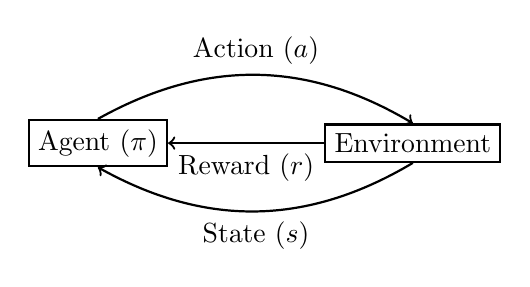
\begin{tikzpicture}[->, thick]
         %nodes
         \node[draw] at (-2,0) (agent) {Agent ($\pi$)}; % : S \to \mathcal{P}(A)
         \node[draw] at (2,0) (env) {Environment};
         \path
             (agent.north) edge[bend left=30] node[above] {Action ($a$)} (env.north)
             (env.south) edge[bend left=30] node[below] {State ($s$)} (agent.south)
             (env.west) edge node[below] {Reward ($r$)} (agent.east);
    \end{tikzpicture}
    % }
    \caption{The general reinforcement learning paradigm.}
    \label{fig:RL}
\end{figure}

The agent decides what actions to perform via a policy function $\pi$, which maps from a state $s \in S$ to either a probability distribution over the action space $\mathcal{P}(A)$ (a ``stochastic policy'') or simply a particular action $a \in A$ (a ``deterministic policy''). Policy functions are typically implemented as neural networks which are then usually optimized using gradient-based methods.

There are a few other common functions used in RL. The \emph{return} at time step $t$ is defined as
\begin{equation}\label{eq:return}
    G_t \defeq \sum_{k=t}^T \gamma^{k-t} R_k, \quad \gamma \in [0,1)
\end{equation}
or the total discounted rewards until the end of the episode at time step $T$. The \emph{state-value function} is the expected return from a particular state while following a policy $\pi$
\begin{equation}\label{eq:state_value}
    v_\pi(s) \defeq \E[G_t | S_t = s]
\end{equation}
Finally, the \emph{action-value function} is the expected return from taking an action $a$ in state $s$, then after following policy $\pi$
\begin{equation}\label{eq:action_value}
    q_\pi(s, a) \defeq \E[G_t | S_t = s, A_t = a]
\end{equation}


\subsection{Action space}

The action space can generally be discrete (there are finitely many actions that can be performed) or continuous  (infinitely many actions). The size of the action space determines the type of RL algorithm that can be used. In discrete action spaces, the policy can be stochastic and learn a probability distribution over every action. In continuous action spaces, where it's impractical to learn an arbitrary probability distribution over all actions, the policy can either be stochastic and learn parameters of a general probability distribution (such as a multivariate Gaussian) or deterministic and return the action.

For Hamiltonian engineering, the size of the action space depends on the number of allowed control Hamiltonians. As an example, in many pulse sequences developed using average Hamiltonian theory, the control Hamiltonians are restricted to $\pi/2$-pulses at consistent time intervals, which is better suited to a discrete action space. In contrast, techniques such as GRAPE
\cite{Khaneja-2005}
allow the control Hamiltonian amplitudes to vary continuously.

Both discrete and continuous action spaces were tested, and the results of each are shared below in the sections for each corresponding RL algorithm.

\subsection{Reward schemes}

The goal of Hamiltonian engineering is to control the system so that its time-evolution appears to be under some effective Hamiltonian. The reward signal should then be larger when the actual evolution is ``close'' to the target evolution. One measure of ``closeness'' is the fidelity function for two unitary operators
\begin{equation} % TODO make sure this is right
    F(U_\text{actual}, U_\text{target}) = \left| \frac{\Tr{
        U_\text{actual}^\dagger U_\text{target}
    }}{\Tr{\identity}} \right|
\end{equation}
The fidelity approaches 1 as the unitaries get closer, and approaches 0 as the unitaries get further apart. However, a tenfold improvement in performance doesn't correspond to a tenfold increase in fidelity (take for instance a fidelity of 0.9 compared to 0.99). A suitable reward function is then calculated by
\begin{equation}
    R = -\log(1-F(U_\text{actual}, U_\text{target}) + \epsilon)
\end{equation}
where $\epsilon>0$ ensures the reward isn't infinite.

There is also the decision of \emph{when} to give rewards to the agent. A reward can be given at every time step during the episode (``dense rewards'') or only at certain time steps such as the end of the episode (``sparse rewards'').
Dense rewards make sense when the fidelity matters at every time step, such as implementing a target unitary in the shortest amount of time possible.
% TODO does ^ make sense? May need to explain more...
Sparse rewards make sense when the fidelity only matters at certain points in time, such as in stroboscopic measurements and pulse sequences.

\subsection{State space and state representation}

The state space is the set of all possible states of the system. A possible approach would be to encode the state as the density matrix or propagator at the current time step. However, the density matrix and propagator grow exponentially as the system size increases, and the complete characterization of the quantum system is unrealistic for any experimental application.

An alternative state representation is the sequence of past actions applied to the system.  This representation generally requires less memory and computation, and may also be better suited to more robust control.

\subsection{Reinforcement learning algorithms}

There are many RL algorithms that have been developed, tailored to the specific characteristics of the problem. The relevant characteristics include
\begin{description}
    \item[Model] An agent in a \emph{model-free} RL algorithm learns a policy directly from observations of the environment. An agent in a \emph{model-based} RL algorithm instead uses observations to model the environment, then uses that model to learn a policy.
    \item[Policy] An \emph{on-policy} algorithm improves the policy that is used to interact with the environment. An \emph{off-policy} algorithm has separate policies for improvement and environment interaction.
    \item[Action space] As mentioned before, an action space can be \emph{discrete} (finitely many actions) or \emph{continuous} (infinitely many actions).
\end{description}
In addition to the above characteristics, there are general classes of RL algorithms, such as temporal-difference learning policy gradient methods. More information on RL can be found in \cite{sutton2018reinforcement}.

\subsubsection{Q-learning and DQN}

Q-learning is a model-free, off-policy, TD control algorithm applicable to discrete action spaces \cite{watkins1989learning}. As the name suggests, the action-value function $Q(s,a)$ is learned from experiences with the environment according to the following update rule
\begin{equation}\label{eq:Q_learning_update}
    Q(S_t, A_t) \leftarrow Q(S_t, A_t) +
        \alpha \left[ R_{t+1} + \gamma \max_a Q(S_{t+1}, a) - Q(S_t, A_t) \right]
\end{equation}
To encourage exploration of the state and action spaces, the agent typically follows an $\epsilon$-greedy policy (with probability $1-\epsilon$ perform the action that maximizes $Q$, otherwise perform a random action), which makes this algorithm \emph{off-policy}.

If the state and action spaces are small, then it's feasible for all the $Q$-values to be stored in memory. In general, though, the action-value function is approximated using a neural network, and the parameters are updated to minimize the loss given by \ref{eq:Q_learning_update}. This approach is called ``deep Q-network'' or DQN \cite{mnih2013playing}. DQN is suitable for large state spaces (as demonstrated through Atari games in \cite{mnih2013playing}), but still requires the action space to be discrete.

\subsubsection{DDPG}

``Deep deterministic policy gradient'' (DDPG) extends the idea of deep reinforcement learning in DQNs to continuous action spaces \cite{lillicrap2015continuous}. As with DQN, DDPG is a model-free, off-policy algorithm, but uses an actor-critic framework that separates the policy and the value function estimators. In addition, the policy is deterministic, so it returns a single action instead of a distribution over actions. As the agent interacts with the environment, the experiences are recorded in a \emph{replay buffer} on which the actor and critic are trained. The critic is updated by minimizing the sampled value estimate errors,
% TODO include update equation?
% \begin{align}\label{eq:DDPG_critic_update}
%     L = \frac{1}{N} \sum_i (y_i - Q(S_i, A_i | \theta^Q))^2 \\
%     y_i = R_i + \gamma Q'(S_{i+1}, \mu'(S_{i+1}|\theta^{\mu'}) |\theta^{Q'})
% \end{align}
and the actor is updated using the sampled policy gradient%
% TODO include?
% \begin{equation}
%     \nabla_{\theta^\mu} J \approx \frac{1}{N} \sum_i
%     \nabla_a Q(s, a | theta^Q)|_{s=s_i, a=\mu(s_i)}
%     \nabla_{\theta^\mu} \mu(s|\theta^\mu)|_{s_i}
% \end{equation}
.

\subsubsection{PPO}

Proximal-policy optimization (PPO) is a model-free, on-policy actor-critic algorithm that tried to improve data efficiency and robustness compared to existing algorithms (such as DQN or other policy gradient methods).
\cite{schulman2017proximal}.
In contrast with other policy gradient methods, the PPO objective function is clipped according to a hyperparameter $\epsilon$.
\begin{equation}\label{eq:ppo_loss}
    % eq 7 in PPO paper
    L(\theta) = \E_t \left[\min(
        r_t(\theta)\hat{A}_t,
        \text{clip}(r_t(\theta), 1-\epsilon, 1+\epsilon) \hat{A}_t
    )\right]
\end{equation}
where
$r_t(\theta) = \frac{\pi_\theta(a_t|s_t)}{\pi_{\theta'}(a_t|s_t)}$ is the probability ratio of actions under the new and old policies, and $\hat{A}_t$ is an estimator of the \emph{advantage function} at time $t$. By clipping the objective, the gradient updates are non-zero only for a region close to the previous policy, thus preventing policy changes that are too large.
PPO has been applied successfully to both continuous and discrete action spaces%
% TODO check above, I think that's right but not sure...
.



\subsubsection{ERL}

Evolutionary reinforcement learning (ERL) is a model-free, off-policy hybrid algorithm that uses both actor-critic policy gradient and evolutionary algorithm methods \cite{khadka2018evolutionguided}. ERL addresses problems found in many  gradient-based RL algorithms, including temporal credit assignment (associating actions to rewards that may be separated by many time steps), exploration of the state and action spaces, and policy convergence sensitivity to hyperparameters. To do so, ERL maintains a population of actors with individual policies that interact with the environment. The population's experiences are recorded in a shared replay buffer, and a separate actor/critic pair learn from the replay buffer using policy gradient (such as DDPG or DQN). Periodically, the policy gradient-based actor is copied into the population, and evolutionary algorithms are used to iterate a new ``generation'' of actors (by preferentially selecting high-performing actors). By using both gradient-based and gradient-free methods, ERL attempts to achieve both efficiency and policy diversity, making it a candidate for a variety of RL problems.

\section{Results}

For the Hamiltonian engineering problem, the lowest-order average Hamiltonian for the WHH-4 pulse sequence was used as the desired effective Hamiltonian
\begin{equation}
    \overline{H}_\text{WHH}^{(0)} = \sum_i
        \frac{\delta_i}{3} \left( \mathbf{I}^i \cdot (1,1,1) \right)
\end{equation}
This removes the dipolar interaction term from the Hamiltonian while retaining the chemical shift term along the $(1,1,1)$ axis.
Many different combinations of RL algorithms, state representations, action representations, and reward schemes have been tested, but none reliably converged to a policy that engineered the desired Hamiltonian.
% TODO write section
% - what I tried to do: AHT-like approach, learn WHH-4 sequence
% - walk through general results, algorithm specifics

% TODO continue here with DQN...

DQN:
\begin{itemize}
\item MATLAB, January-March
\item May(ish), started using TF-Agents
\item Algorithm learned to delay only, not sufficient exploration in state
  space
\end{itemize}

PPO
\begin{itemize}
\item Similar to DQN, generally learned to delay or to rotate back and forth
\end{itemize}

ERL
\begin{itemize}
\item most success using this algorithm, but it's construction promotes more
  exploration and diversity of policies
\end{itemize}

\section{Conclusions}

% TODO

\begin{itemize}

\item RL is hard

  \begin{itemize}
  
  \item Non-stationary nature of problem (training model on data generated
    by model) is difficult
  \item Balancing exploration and exploitation
  \item Discontinuous reward function on state space
  \end{itemize}
\item Distinguishing between working algorithm and luck (esp.~with ERL)
\end{itemize}

% TODO next steps

\begin{itemize}

\item Look more into supervised learning

  \begin{itemize}
  
  \item Learn map from pulse sequence to fidelity
  \item Learn map from pulse sequence to average Hamiltonian
  \end{itemize}
\item Consider continuous action space

  \begin{itemize}
  
  \item Less a combinatorial problem, closer to existing applications of RL
  \end{itemize}
\end{itemize}

\bibliography{../refs.bib}

\end{document}
